\documentclass{article}
\usepackage{v-problem}
\vgeometry

\begin{document}
\vtitle[ELECTROSTATICS]

\def\pn{06}
\def\book{Irodov}
\def\page{106}
\def\gdrive{https://drive.google.com/drive/folders/1hWY2Kys1IyA1slYM0qPtR9pjIDTu7LUd?usp=share_link}

\def\question{
A thin wire ring of radius $r$ has an electric charge $q$. What will be the increment of the force stretching the wire if a point charge $q_0$ is placed at the ring's centre?
}

\vspace*{\fill}
\begin{tikzpicture}
	\node[qnumber] (n) at (0, 0)[scale=2] {$\pn.$};
	\node[question] (q) [right=2mm of n.east] {\question};
	\tzline[divider]<-0.125, 0> (q.north west)(q.south west);
	\node[format] (f) at  (q.south east){[\book \quad \page]};
\end{tikzpicture}	
\vspace*{\fill}

\begin{center}
\begin{tikzpicture}
\tzcoor*(0, 0)(O){$q_0$}[bl](5pt)
	\foreach \a in {0, 8, ..., 352}{
		\tznode(\a:2){$+$}[scale=0.65]
		\tzdot[thin](\a:2)(6pt)	
	}
	\tznode($(O)+(0, -2.1)$){$q$}[b]
	\tzline[->, thick](O)(40:2){$r$}[mb]
\end{tikzpicture}
\end{center}

\vspace*{\fill}
\pagebreak

\vtitle[\texttt{Solution}]
\begin{center}
\begin{tikzpicture}
	\foreach \a in {0, 8, ..., 352}{
		\tznode(\a:2){$+$}[scale=0.65]
		\tzdot[thin](\a:2)(6pt)
		\ifthenelse{\a=0}{}{
			\tzline[->]($(\a:2)!0.11cm!(0:2)$)($(\a:2)!4.5cm!(0:2)$)
		}	
	}
\end{tikzpicture}
\end{center}
\textit{This is how every element will experience a net outward force due to other elements on the ring. This will cause a tension in the ring.}
\pagebreak

\begin{center}
\begin{tikzpicture}
[thick]
\def\A{16} %angle for element
\def\r{2} %radius
\def\dr{0.1} %delta r
\def\RO{\r+\dr} %radius outer
\def\RI{\r-\dr} %radius inner
\tzcoor(0:\RO)(O') %point at right end
\tzcoor*(0, 0)(O){$q_0$}[bl](5pt)
	\foreach \a in {0, 8, ..., 352}{
		\tznode(\a:\r){$+$}[scale=0.65]
		\draw[thin](\a:\r) circle [radius=\dr];
	}
	\tzlines(O)(\A:\RO)(O)(-\A:\RO);
	\tzarc(O)(-\A:\A:\RO)
	\tzarc(O)(-\A:\A:\RI)
	\tzline[->](\A:\RO)($(\A:\RO)!2cm!(1.01*\A:\RO)$){$\Delta T$}[a]
	\tzline[->](-\A:\RO)($(-\A:\RO)!2cm!(-1.01*\A:\RO)$){$\Delta T$}[b]
	\tzline+[->](O')(2, 0){$\Delta F_e$}[r]
	\tzanglemark'(-\A:\r)(O)(\A:\r){$\d{\theta}$}(15pt)
	\tzline[<->, thick]($(O')+(0,2.5)$)($(O')+(0,-2.5)$)
	\tzarc[thick](O')(90:90+0.7*\A:1){$\d{\theta}/2$}[a=2mm, r=1mm]
	\tzarc[thick](O')(270-0.7*\A:270:1)
\end{tikzpicture}
\end{center}
\textit{Placing a charge $q_0$ at the center will further increase the outward force on every element hence the tension.\\[5mm]
We have to find this extra tension($\Delta T$) caused by $q_0$. 
}

\pagebreak

\def\K{\dfrac{1}{4\pi\varepsilon_0}}
\addtolength{\jot}{3ex}
\begin{align*}
\intertext{Vertical components of $\Delta T$ will get concelled out.}
\intertext{Horizontal components($2\Delta T \sin\left(\d{\theta}/2\right)$) will get balanced by $\Delta F_e$}
2 \cdot \Delta T \cdot \sin\left(\dfrac{\d{\theta}}{2}\right) &= \Delta F_e\\
\intertext{As $\d{\theta}$ too small $\sin\theta \rightarrow \theta$}
2 \cdot \Delta T \cdot \left(\dfrac{\d{\theta}}{2}\right) &= \K \cdot \dfrac{\lambda \cdot r \cdot \d{\theta} \cdot q_0}{r^2} \\
\Delta T \cdot \d{\theta} &= \K \cdot \dfrac{\dfrac{q}{2\pi r} \cdot r \cdot \d{\theta} \cdot q_0}{r^2} \\
\Delta T &= \dfrac{qq_0}{8\pi^2\varepsilon_0 r^2} \ans
\end{align*}

\pagebreak

\vspace*{\fill}
\begin{center}
	\fbox{\qrcode[height=2cm]{\gdrive}}
\end{center}
\vspace*{\fill}

%\pagebreak
%\begin{center}
%\tdplotsetmaincoords{70}{120}
%\begin{tikzpicture}
%[tdplot_main_coords, fill opacity=0]
%\tdplotsetpolarplotrange{0}{180}{120}{150}
%\tdplotsphericalsurfaceplot[parametricfill]{36}{18}%
%{1}{black!75}{\tdplotphi + 3*\tdplottheta}
%    {\tzline[->](0, 0, 0)(3, 0, 0){$x$}[b]}%
%    {\tzline[->](0, 0, 0)(0, 3, 0){$y$}[r]}%
%    {\tzline[->](0, 0, 0)(0, 0, 3){$z$}[r]}%
%\end{tikzpicture}
%\end{center}


\end{document}
